
\documentclass[a4, 10pt,dvipdfmx,twocolumn]{jsarticle}

%\usepackage[chukan]{sotsuron}
%\usepackage[dvips]{graphicx}

%\setlength{\topmargin}{-13truemm}
%\setlength{\headheight}{0mm}
%\setlength{\headsep}{0mm}
%\setlength{\textheight}{45\baselineskip}
%\setlength{\textheight}{26cm}
%\addtolength{\textheight}{\topskip}
%\addtolength{\textwidth}{5cm}
%\addtolength{\oddsidemargin}{-2.5cm}

\usepackage[dvipdfmx]{graphicx}
\def\pgfsysdriver{pgfsys-dvipdfmx.def}
\usepackage{threeparttable}
\usepackage{tikz}
\usepackage[chukan, nobroaderlayout]{sotsuron}
% \usepackage[chukan]{sotsuron}
\usepackage{ascmac}
\usepackage{bm}
\usepackage{amsmath}
\usepackage{fancybox}
\usepackage{url}

\title{モンテカルロ木探索を用いた交渉の評価関数の提案}
\author{東京大学工学部電子情報学科 近山•鶴岡研究室 4年 伊藤 義章}
\date{2013年2月17日}

\begin{document}
 % \makecover

\pagenumbering{roman}

 % \tableofcontents

\newpage
\maketitle

\pagenumbering{arabic}

\section{目的と背景}

実世界では、競争的状況において自分の利益を最大化することを目指した多くの交渉が行なわれている。交渉に関する研究の多くは、交渉の定性的な研究であり、交渉の定量的な側面に着目した研究は未だ発展途上である。その理由のひとつは、交渉によって得られる可能性のある利益を数値化し、どのような交渉を提示するかの指標となる評価関数を用意することの難しさにある。本研究では、交渉において重要となる要素を定量的な観点から明らかにする事を目的とし、利益の数値化の方法として、行動の先読みおよび評価関数を用いる事を提案する。
具体的には、先読みによる利益計算に、近年成功をおさめているモンテカルロ法を用いることを提案し、また、利益計算の指標となる様々な評価関数を提示する。

\section{関連研究}
\subsection{UCTアルゴリズム (UCB applied to Trees)}
状態の評価が難しい問題において有効とされる手法としてモンテカルロ法がある。
ある局面から終局までランダムに行われる試行(プレイアウトと呼ばれる)に基づき、候補手を統計的に評価する。
% プレイアウトを繰り返す事で、ある局面の勝率を計算することができる。
しかし、時間が有限の場合、明らかに有望でない手に対して、有望な手と同様の試行回数を行うべきではない。UCTアルゴリズムは、有望な手にUCB値 (Upper Confidence Bound、以下 UCB)\cite{kocsis2006bandit}を用いてバイアスをかけるモンテカルロ木探索である。
% 子ノードを選択する場合、まず未探索の子ノードを優先的に選択する。
% 子ノードが全て探索済みの場合は、探索回数が少なく、高い報酬を得る可能
% 性のある手を優先的に選択する。
% 選択したノードをプレイアウトした後は、その結果を報酬として探索経路上のノードに更新する。
% 以上の
UCTアルゴリズムは、「子ノードの選択」「子ノードの展開」「プレイアウト」「結果の更新」を終了条件 (時間や探索回数など) となるまで繰り返し、平均報酬の最も高い子ノードを選択する。
% UCTアルゴリズムは、カタンのAIであるSmartSettlersに適用させ、成功をおさめている\cite{szita2010monte}。他の3人ランダムプレイヤーに対し、プレイアウト回数を0回、1000回、10000回として対戦した結果、25\%、27\%、49\% の勝率を残し、カタンにおけるモンテカルロ木探索がランダムプレイヤーよりは強いことを示している。
% \begin{figure}[b]
%     \begin{center}
%       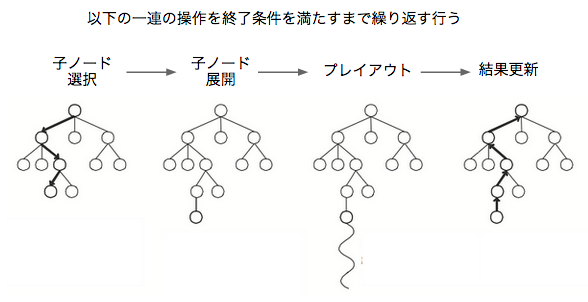
\includegraphics[width=80mm]{img/monte_carlo.png}
%     \end{center}
%     \caption{モンテカルロ木探索~\cite{kocsis2006bandit}}
%     \label{monte_carlo}
% \end{figure}

\subsection{交渉のアルゴリズム}
交渉決裂により、実際に得られるはずだった利益を得られず、機会損失を招いてしまう。
交渉案を選択する評価関数の機会損失を図る指標として譲歩率がある\cite{baarslag2012evaluating}。
ANACにて優秀とされる結果を残した人工知能のIAMhaggler2011\cite{baarslag2012evaluating}は、一定の譲歩を行なっていることから、自分の利益のみを考える評価関数が優位な戦略でないと考えられる。


% 妥協点を見つける方法として、相手のモデル化\cite{baarslag2012evaluating}がある。例えば、IAMhaggler2011は序盤の交渉でガウス過程的\cite{rasmussen2006gaussian}にモデル化を行なう事で、相手の利益を予測することができる。これを適用したIAMhaggler2011\cite{williams2013iamhaggler2011}とい人工知能は、ANAC(Automated Negotiating Agents Competition、以下ANAC)にて優秀な結果を残している。IAMhaggler2011は相手の利益を予測した後、自分の利益を最大化する交渉案が最もよい結果を残している。

% また、交渉案を選択する評価関数の譲歩率を測定する方法\cite{baarslag2012evaluating}がある。譲歩率は機会損失をさける指標となる。
% ANACにて優秀とされる結果を残した人工知能のIAMhaggler2011\cite{baarslag2012evaluating}は、一定の譲歩を行なっていることから、自分の利益のみを考える評価関数が優位な戦略でないと考えられる。

\section{提案手法}
\subsection{利益の見積もり}
UCTアルゴリズムの先読みによって得た勝率を、利益計算に用いる事にする。プレイアウトを行なう事で、各プレイヤーの勝率を計算することができる。交渉による損得は勝率に直結することから、UCTアルゴリズムの先読みによって予め得た勝率により利益計算を行なうことができると考えられる。

\subsection{評価関数の作成}
本研究では、前節で得られた利益計算の結果を用いて、交渉の成功率を考慮した評価関数を用いて各交渉の期待値を求める。
ただし、交渉の成功率は「相手が得られる利益」に影響を受けるものだと仮定する。
良い交渉案を選ぶ評価関数として、以下の5つの評価方法を提案する。
まず、自分の利益のみしか考えない「自己中心的交渉」を行なうプレイヤーをベースラインとして扱う。次に、相手の利益を優先にした「利益優先交渉」と交渉の成功率を優先した「受諾優先交渉」を提示する。また、お互いの利益をバランスよく配分する手法として、「和交渉」「積交渉」を提示する。


\section{評価}
\subsection{UCTの利益計算}
ルールベースプレイヤーは全受諾プレイヤーに対して42.1\%とベースラインであるランダムプレイヤーに41.25\%と有意な実力差を示したことから、自分にとって有利となる利益計算を行い、交渉案を提示していることが分かる。
一方で、UCTプレイヤーは受諾プレイヤーに対して23.6\%、ランダムプレイヤーに25.0\%と有意な実力差を得られなかった。
ルールベースと交渉選択の一致率を検証した結果、要因として「プレイアウト回数が不十分であったこと」「相手の勝率が高くなった場合での精度悪化」が考えられる。

\subsection{評価関数}


\begin{figure}[h]
    \begin{center}
      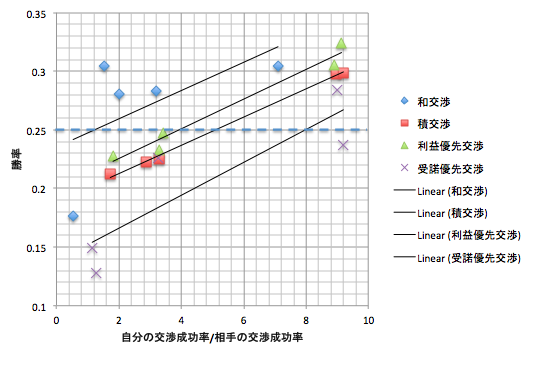
\includegraphics[width=80mm]{img/relation_winrate.png}
    \end{center}
    \caption{評価関数の勝率と交渉成功率}
    \label{win_rate}
\end{figure}


図より、全ての評価関数において(自分の交渉成功率/相手の交渉率)の割合が高まれば高まるほど良い勝率を残すことができると考えられる。このことからも、交渉における「提案成功率」と「受諾率」が関係していると考えられる。また、和交渉ではばらついたものの、利益優先交渉や、積交渉のように近似直線を描くと一定の直線上にのっていることがわかる。また、図よりこれら4つの直線の傾きは一定であるが、評価関数によってその近似直線が上下することがわかる。評価関数によって近似直線が上下する原因として、「自分にとっての利益」と「相手に与える損益」のバランスによるものと考えられる。バランス型の交渉である和交渉では、相手に与える損益を加えたことが高い勝率に結びついたと考えられる。また、受諾優先交渉、利益優先交渉と積交渉では相手に与える損益がないため、自分の得られる利益が大きい順に高い結果を残すことができたと考えられる。利益優先や受諾優先ではなくバランスよく利益配分を行なう和交渉がもっともよい結果を残したことから、「自分にとっての利益」と「相手に与える損益」をバランスよく配分する評価関数が最もよい評価関数だと考えられる。

交渉の評価関数において「提案成功率」「受諾率」「自分の利益」「相手の損益」が重要な要素であると明らかにした。「相手の損益」を考慮するのは、自分では悪い交渉案だと思っている交渉案においても、相手との評価基準が自分よりもずれていることを利用して、悪い交渉案を混ぜることで勝率を高めることができると考えられるためである。




\section{おわりに}

% 本論文では、交渉の利益計算手法をルールベースとUCTアルゴリズムの2つを提案し、UCTアルゴリズムの交渉への適用を試みた。また、交渉の評価関数を5つ提案し、対戦実験を行なう事で、交渉における4つの要素を明らかにした。
% UCTアルゴリズムによる利益計算はプレイアウトによる勝率のフィードバックを用いることにより行なった。受諾プレイヤーに対して有意に高い勝率を残したルールベースプレイヤーと交渉案の一致率を確認することにより、UCTアルゴリズムによる利益計算の問題点を明らかにした。
% 交渉の評価関数において「提案成功率」「受諾率」「自分の利益」「相手の損益」が重要な要素であると明らかにした。相手の損益」を考慮するのは、自分では悪い交渉案だと思っている交渉案においても、相手との評価基準が自分よりもずれていることを利用して、悪い交渉案を混ぜることで勝率を高めることができると考えられるためである。

\subsection{まとめ}
% 利益見積もりに、UCTを用いた先読みより得られた評価値また、今回シミュレーションを行うJSettlersの交渉時における挙動を確認できるため、今後の交渉相手として交渉を受け入れるプレイヤーであるかを確認できると期待される。

先読みによる利益計算に、近年成功をおさめているモンテカルロ法を用いることを提案し、また、利益計算の指標となる様々な評価関数を提示した。不確定不完全情報ゲームである「カタンの開拓者」をテストベッドとして実験を行なった結果、利益計算におけるモンテカルロ法の有効性を示す事はできなかった。しかし、交渉の評価関数を作成する上で、「提案成功率」「受諾率」「自分の利益」のみならず、「相手の損益」を考慮した評価関数を作成する必要があることを明らかにした。

\subsection{今後の課題}
利益見積もりを改善するため、UCTアルゴリズムのプレイアウト回数を向上することと、極端な局面でのバイアスを導入することがある。プレイアウト時間は線形に増加してしまうことから、一定の時間でシミュレーションを打ち切り、評価関数を用いて盤面を評価し、その時点で評価値が最も高いプレイヤーを暫定の勝利者とするといった工夫が必要となる。


\bibliographystyle{jplain}
\bibliography{chukan_presentation}

 \end{document}
